\section{Introduction} \label{sec:Introduction}

\begin{comment}
idé gør som Cochrane og Campbell 1999:
\begin{enumerate}
    \item Kalibrer modellen (Mikrofundament)
    \item Simulér variable og PD
    \item Lav Recesssionsdummy fra surplus consumption / consumption
    \item Cross-sectional regressions med dummies
    \item Kan man forecaste OoS returns under recession og ikke expansion <- theoretical
\end{enumerate}

\hline

\begin{enumerate}
    \item evidence for predictability in recessions is already established, however due to the fact that the state of the economy only is recession approximately 10\% of the time, we find it interesting to investigate the power of the model in expansions as well. 
    \item This investigation will be conducted relaying heavily upon \cite{Campbell1999} and using a regime switchin regression framework. 
    \item The recession dummy will be construted from the surplus consumption ration simple as follows
    \begin{align}
        rec_t & = \begin{cases} 1 & \text{, if } s_t < \Bar{s} \\
                              0 & \text{, if } s_t > \Bar{s} \end{cases}
    \end{align}
    
    and the regression equation below
    
    \begin{align}
        r_{t+h} & = \alpha + \beta_1 \times r_t + \underbrace{\beta_2 \times pd_t  \times I_{rec_t}}_{\text{recession indicator}} + \underbrace{\beta_3 \times pd_t \left(1 - I_{rec_t} \right)}_{\text{Expansion Indicator}} + \varepsilon_{t+h} 
    \end{align}
    
    skriv noget om hvad andre har fundet ud af, nævn stigs 2013 artikel ifm. bond return predictability og nævn andre campbel osv der finder unpredictability i returns.

\end{enumerate}




This paper investigates the Habit Formation model proposed by \cite{Campbell1999} ability to predict in expansions as well as the out-of-sample performance of the model. 
The history of Asset Pricing models have provided evidence of predictability in periods of economic downturn \colorbox{yellow}{\textbf{INDSÆT KILDER}}, however, there have been little evidence showing predictability in expansions. The ability to predict in expansions are a highly desired capability, due to the fact the economy historically is in the state of expansion more often than recession. In the \cite{Campbell1999} framework, recession is defined as period where surplus consumption is below steady-state, hence the models recession is not exactly equal to the definition of three quarters of negative GDP growth as we are used to...


\hline

We examine the \cite{Campbell1999} model of Habit formation in asset pricing. Investigating the models performance both in recessions, which multiple sources have provided evidence of predictability of returns, and in expansions where it has been the case to be more difficult to predict returns. 

We calibrate the model based on newer data than \cite{Campbell1999}, then we perform a simple regression with an indicator variable of recession and $(1-I_{rec}$ for expansions, this is done for the ability to distinguish between model performance in recessions as well as in expansions. 

A recession in the model is defined as when surplus consumption is below some given value, that is 

    \begin{align}
        I_{rec} & = \begin{cases} 1 & \text{, if } s_t < s_{rec} \\
                                  0 & \text{, if } s_t > s_{rec} 
                    \end{cases}
    \end{align}

in order to match the empirical amount of times the economy have been in recession according to \cite{USREC} in the period $1950 - 2018$ $\approx 13 \%$, the threshold $s_{rec}$ needs to take a value somewhere below $s_{bar}$, otherwise if $s_{bar}$ is used as threshold the economy of the model will be in recession approximately $37\%$ of the time, this three times more than the economy actually have been in the last 68 years, thus the need for lowering the threshold. The threshold value of the surplus consumption ratio is found by integrating over the stationary distribution of the surplus consumption ratio.


 \begin{figure}[H]
    \centering
    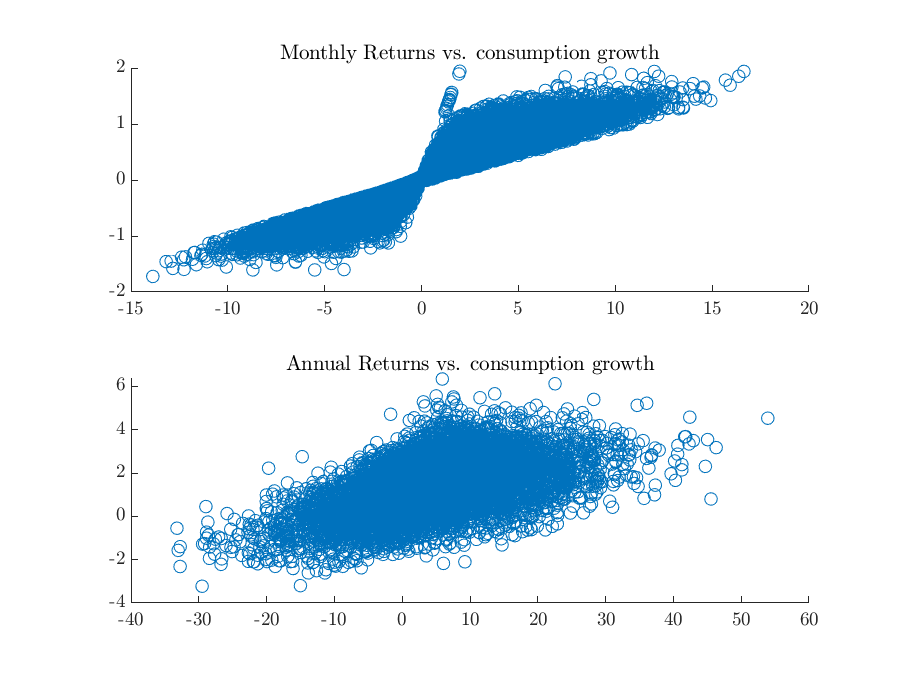
\includegraphics[width=0.5\textwidth]{Code_v2/Figures/Figure_7_CC_1998.eps}
    \caption{\cite{Campbell1999} figure 7}
    \label{fig:CC1998_fig_7}
 \end{figure}
 
  \begin{figure}[H]
    \centering
    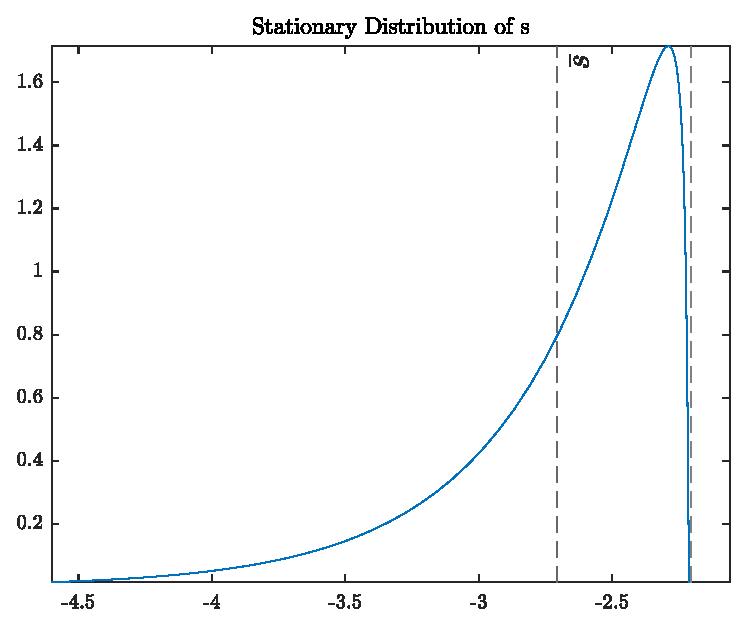
\includegraphics[width=0.5\textwidth]{Code_v2/Figures/Stationary_Density.eps}
    \caption{Stationary Density of surplus consumption}
    \label{fig:Stationary_Density}
 \end{figure}
 
   \begin{figure}[H]
    \centering
    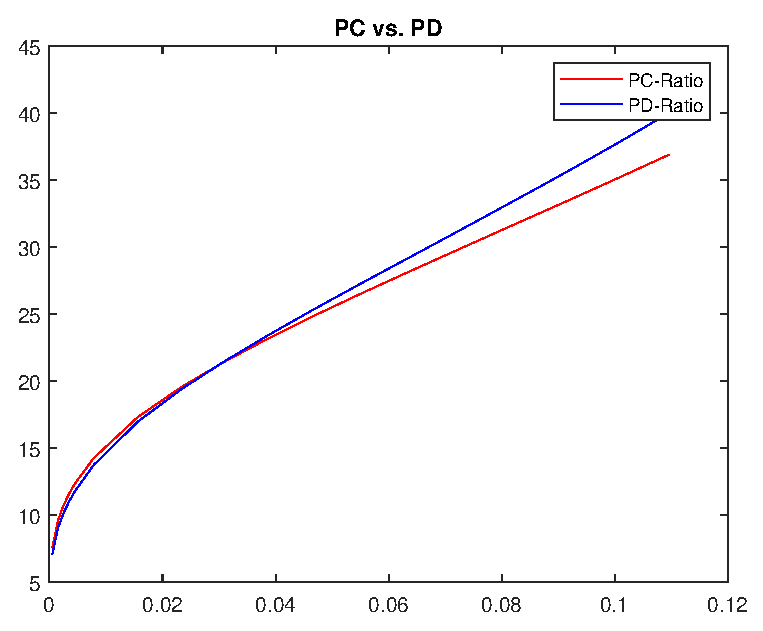
\includegraphics[width=0.5\textwidth]{Code_v2/Figures/PC_PD_ratio.eps}
    \caption{PC \& PD ratio}
    \label{fig:PC_PD_Ratio}
 \end{figure}

\clearpage

\end{comment}


Predictability of asset prices in expansions is a desirable capability since the economy is in a state of expansion more often than recession. In the period $1950-2018$\footnote{According to \cite{USREC}} the economy has been in recession $13.41\%$ of the time, hence being able to predict asset prices in expansions would yield a higher profit for investors.

We show that returns are predicable in recession but unpredictable in expansions. We simulate an economy according to \cite{Campbell1999}, and recalibrate the parameters of model to an extended period $\left(1950-2018\right)$ compared to \cite{Campbell1999} $\left(1950-1994 \right)$, this might catch relevant information in our recalibration since due to the recession in 2000 and the Great Financial Crisis (GFC) of 2008, that is not present in \cite{Campbell1999} calibration.



\subsection{Habit Formation} 

\subsection{Literature Review}


